\documentclass[svgnames,table,,aspectratio=169]{beamer}
%\documentclass[svgnames,table,handout,aspectratio=129]{beamer}
\usepackage{hhline}
\usepackage{etoolbox}
\usepackage{tikz}
\usepackage{mathtools}
\usepackage{amssymb}
%\usepackage{/usr/lib64/R/share/texmf/Sweave}
\usepackage{polynom}
\usepackage{qrcode}


%\input{latexdefinitions}
\definecolor{georgiaRed}{RGB}{100,0,00}
\definecolor{mediumGray}{gray}{0.6}



\usetheme{Frankfurt}%
%\usetheme{Warsaw}%
%\useoutertheme{smoothbars}


%\usecolortheme{seagull}
\usecolortheme{beaver}
\logo{\includegraphics[height=.125in]{ugaLogo}}

% Note that the colour definitions are given in the latexDefinitions
% file.
\setbeamercolor{palette primary}{fg=georgiaRed,bg=white}
\setbeamercolor{palette secondary}{fg=georgiaRed,bg=white}
\setbeamercolor{palette tertiary}{fg=georgiaRed,bg=white}
\setbeamercolor{palette quaternary}{bg=mediumGray,fg=black}
\setbeamercolor{block title}{fg=white,bg=georgiaRed}
\setbeamercolor{block body}{fg=black,bg=black!10}
\setbeamercolor{titlelike}{bg=georgiaRed,fg=white} % parent=palette quaternary}

% Define the variable to determine whether or not the clicker quizzes
% are visible in the resulting output.
\newtoggle{clicker}
\toggletrue{clicker}
%\togglefalse{clicker}


% To display a lecture uncomment out the "includeonly" line below to
% match the name of the file. You do not have to do anything with the
% lecture line below and can leave it commented out. It is in place
% because at one time we had multiple lectures within a file, but that
% has been changed.



\mode<presentation>{
  \setbeamercovered{invisible}
  \setbeameroption{hide notes}
}

\mode<handout>{
 
  \usepackage{pgfpages}
  %\pgfpagesuselayout{4 on 1}[letterpaper, border shrink=5mm]
  \pgfpagesuselayout{resize to}[letterpaper,border shrink=5mm]
  \setbeameroption{show notes}


  %\pgfpagesphysicalpageoptions{logical pages=2,physical
  %height=\pgfpageoptionheight,physical width=\pgfpageoptionwidth}
  % Set up the pages for notes.
  % This idea and some code came from
  % http://www.guidodiepen.nl/2009/07/creating-latex-beamer-handouts-with-notes/



  \pgfpagesdeclarelayout{3 on 1 with notes} {
    \edef\pgfpageoptionheight{11in} %\the\paperheight}
    \edef\pgfpageoptionwidth{8.5in} %\the\paperwidth}
    \edef\pgfpageoptionborder{0pt}
  }

  {

	\AtBeginDocument{
      \newbox\notesbox
      \setbox\notesbox=\vbox{
        \hsize=\paperwidth
        \vskip-2.5cm\hskip-5cm\vbox{
          \textcolor{light-gray}{\hrule width 12.6cm\vskip0.5cm}
          \textcolor{light-gray}{\hrule width 12.6cm\vskip0.5cm}
          \textcolor{light-gray}{\hrule width 12.6cm\vskip0.5cm}
          \textcolor{light-gray}{\hrule width 12.6cm\vskip0.5cm}
          \textcolor{light-gray}{\hrule width 12.6cm\vskip0.5cm}
          \textcolor{light-gray}{\hrule width 12.6cm\vskip0.5cm}
          \textcolor{light-gray}{\hrule width 12.6cm\vskip0.5cm}
          \textcolor{light-gray}{\hrule width 12.6cm\vskip0.5cm}
          \textcolor{light-gray}{\hrule width 12.6cm\vskip0.5cm}
          \textcolor{light-gray}{\hrule width 12.6cm\vskip0.5cm}
          \textcolor{light-gray}{\hrule width 12.6cm\vskip0.5cm}
          \textcolor{light-gray}{\hrule width 12.6cm\vskip0.5cm}
          \textcolor{light-gray}{\hrule width 12.6cm\vskip0.5cm}
          \textcolor{light-gray}{\hrule width 12.6cm\vskip0.5cm}
          \textcolor{light-gray}{\hrule width 12.6cm\vskip0.5cm}
          \textcolor{light-gray}{\hrule width 12.6cm\vskip0.5cm}
          \textcolor{light-gray}{\hrule width 12.6cm\vskip0.5cm}
          \textcolor{light-gray}{\hrule width 12.6cm\vskip0.5cm}
          \textcolor{light-gray}{\hrule width 12.6cm\vskip0.5cm}

          \vspace*{-9.75cm}
          \textcolor{light-gray}{\rule[-1.0cm]{1pt}{9.25cm}\hskip0.5cm}
          \textcolor{light-gray}{\rule[-1.0cm]{1pt}{9.25cm}\hskip0.5cm}
          \textcolor{light-gray}{\rule[-1.0cm]{1pt}{9.25cm}\hskip0.5cm}
          \textcolor{light-gray}{\rule[-1.0cm]{1pt}{9.25cm}\hskip0.5cm}
          \textcolor{light-gray}{\rule[-1.0cm]{1pt}{9.25cm}\hskip0.5cm}
          \textcolor{light-gray}{\rule[-1.0cm]{1pt}{9.25cm}\hskip0.5cm}
          \textcolor{light-gray}{\rule[-1.0cm]{1pt}{9.25cm}\hskip0.5cm}
          \textcolor{light-gray}{\rule[-1.0cm]{1pt}{9.25cm}\hskip0.5cm}
          \textcolor{light-gray}{\rule[-1.0cm]{1pt}{9.25cm}\hskip0.5cm}
          \textcolor{light-gray}{\rule[-1.0cm]{1pt}{9.25cm}\hskip0.5cm}
          \textcolor{light-gray}{\rule[-1.0cm]{1pt}{9.25cm}\hskip0.5cm}
          \textcolor{light-gray}{\rule[-1.0cm]{1pt}{9.25cm}\hskip0.5cm}
          \textcolor{light-gray}{\rule[-1.0cm]{1pt}{9.25cm}\hskip0.5cm}
          \textcolor{light-gray}{\rule[-1.0cm]{1pt}{9.25cm}\hskip0.5cm}
          \textcolor{light-gray}{\rule[-1.0cm]{1pt}{9.25cm}\hskip0.5cm}
          \textcolor{light-gray}{\rule[-1.0cm]{1pt}{9.25cm}\hskip0.5cm}
          \textcolor{light-gray}{\rule[-1.0cm]{1pt}{9.25cm}\hskip0.5cm}
          \textcolor{light-gray}{\rule[-1.0cm]{1pt}{9.25cm}\hskip0.5cm}
          \textcolor{light-gray}{\rule[-1.0cm]{1pt}{9.25cm}\hskip0.5cm}
          \textcolor{light-gray}{\rule[-1.0cm]{1pt}{9.25cm}\hskip0.5cm}

        }

      }

    \pgfpagesphysicalpageoptions
    {%
      logical pages=6,%
      physical height=\pgfpageoptionheight,%
      physical width=\pgfpageoptionwidth,%
      last logical shipout=3%
    }
    
    \pgfpageslogicalpageoptions{1}
    {%
      border shrink=\pgfpageoptionborder,%
      resized width=.5\pgfphysicalwidth,%
      resized height=.33\pgfphysicalheight,%
      center=\pgfpoint{.25\pgfphysicalwidth}{.82\pgfphysicalheight}%
    }%
    \pgfpageslogicalpageoptions{2}
    {%
      border shrink=\pgfpageoptionborder,%
      resized width=.5\pgfphysicalwidth,%
      resized height=.33\pgfphysicalheight,%
      center=\pgfpoint{.25\pgfphysicalwidth}{.47\pgfphysicalheight}%
    }%
    \pgfpageslogicalpageoptions{3}
    {%
      border shrink=\pgfpageoptionborder,%
      resized width=.5\pgfphysicalwidth,%
      resized height=.33\pgfphysicalheight,%
      center=\pgfpoint{.25\pgfphysicalwidth}{.17\pgfphysicalheight}%
    }%	
	\pgfpageslogicalpageoptions{4}
    {%
      border shrink=\pgfpageoptionborder,%
      resized width=.5\pgfphysicalwidth,%
      resized height=.33\pgfphysicalheight,%
      center=\pgfpoint{.85\pgfphysicalwidth}{.82\pgfphysicalheight},%
      copy from=4
    }%
    \pgfpageslogicalpageoptions{5}
    {%
      border shrink=\pgfpageoptionborder,%
      resized width=.5\pgfphysicalwidth,%
      resized height=.33\pgfphysicalheight,%
      center=\pgfpoint{.85\pgfphysicalwidth}{.47\pgfphysicalheight},%
      copy from=5
    }%
    \pgfpageslogicalpageoptions{6}
    {%
      border shrink=\pgfpageoptionborder,%
      resized width=.5\pgfphysicalwidth,%
      resized height=.33\pgfphysicalheight,%
      center=\pgfpoint{.85\pgfphysicalwidth}{.17\pgfphysicalheight},%
      copy from=6
    }%
    
      \pgfpagesshipoutlogicalpage{4}\copy\notesbox
      \pgfpagesshipoutlogicalpage{5}\copy\notesbox
      \pgfpagesshipoutlogicalpage{6}\copy\notesbox
    }
  }

  \pgfpagesuselayout{3 on 1 with notes}

}

\setbeamercolor{upper separation line head}{bg=red}
\setbeamercolor{headline}{bg=red}
\setbeamertemplate{headline}
{%
\begin{beamercolorbox}{section in head/foot}
\insertsectionnavigationhorizontal{.75\textwidth}{}{}
\hfill \insertpagenumber /\insertdocumentendpage
\end{beamercolorbox}%
}
\setbeamercolor{section number projected}{bg=red,fg=black}
\setbeamercolor{subsection number projected}{bg=red,fg=black}
%\setbeamercolor{frametitle}{bg=lightgray,fg=black}

\setbeamertemplate{itemize item}{\color{georgiaRed}$\blacklozenge$}
\setbeamertemplate{itemize subitem}{\color{georgiaRed}$\blacktriangleright$}

\newcommand{\dotfield}[2]{%
  \begin{tikzpicture}[y=0.25cm, x=0.25cm,font=\sffamily]
    \foreach \y in {0,...,#2} {
      \foreach \x in {0,...,#1} {
        \draw[fill=georgiaRed,opacity=0.1] (\x,\y)  circle [radius=0.03em];
      }
    }
  \end{tikzpicture}
}

\newcommand{\twoByTwo}[4]{%
  \left[
    \begin{array}{rr}
      #1 & #2 \\
      #3 & #4 \\
    \end{array}
  \right]
}

\newcommand{\threeByThree}[9]{%
  \left[
    \begin{array}{rrr}
      #1 & #2 & #3 \\
      #4 & #5 & #6 \\
      #7 & #8 & #9
    \end{array}
  \right]
}

\newcommand{\columnVector}[1]{%
  \left[
    \begin{array}{r}
    #1                           
    \end{array}
  \right]
}

\newcommand{\Tr}{\mathrm{Tr}}

\begin{document}



\author{\textsc{T. Alli$^{a}$, K. Black$^{a}$}}
\institute{$^a$Department of Mathematics, University of Georgia, GA}
\subject{Linear Algebra}
\keywords{Linear Transformation, Vectors, Matrices, Linear Algebra}

%\lecture{Partial Fractions}{partial-fractions}
%\section{Rational Functions}

\title{Section 5.2: The Characteristic Polynomial}
\subtitle{Determining The Eigenvalues Of A Matrix}


\date{} % {\today}

\begin{frame}
  \titlepage
\end{frame}

\begin{frame}{Outline}
  \tableofcontents
\end{frame}


\section{Goals}

\begin{frame}{Goals}

  \begin{itemize}
  \item Determine the characteristic polynomial of a matrix.
  \item Determine the eigenvalues of a matrix using the characteristic
    polynomial.
  \item Factor the characteristic polynomial efficiently to determine
    the eigenvalues of a matrix.
  \end{itemize}

\end{frame}

\section{The Characteristic Polynomial}

\begin{frame}{Example: Determine The Eigenvalues}

  Determine the eigenvalues of the matrix
  \begin{eqnarray*}
    A & = & \twoByTwo{-28}{-30}{24}{26}
  \end{eqnarray*}

  \uncover<2->{$\lambda^2+2\lambda-8$}

  \dotfield{60}{24}
  
\end{frame}

\begin{frame}{The Characteristic Polynomial}

  \begin{block}{Definition: The Characteristic Polynomial}
    Given an $n\times n$ matrix, $A$, the characteristic polynomial of
    the matrix is $\det\left(A-\lambda I_n\right)$.
  \end{block}

\end{frame}

\begin{frame}{Example}

  Determine the characteristic polynomial of the matrix
  \begin{eqnarray*}
    B & = & \threeByThree{1}{-1}{-1}{6}{10}{6}{-9}{-11}{-7}.
  \end{eqnarray*}

    \begin{columns}
      \column{0.3\textwidth}
      \only<2->{$$-\lambda^3 + 4\lambda^2+4\lambda-16$$}

      \column{0.7\textwidth}
      \only<3>{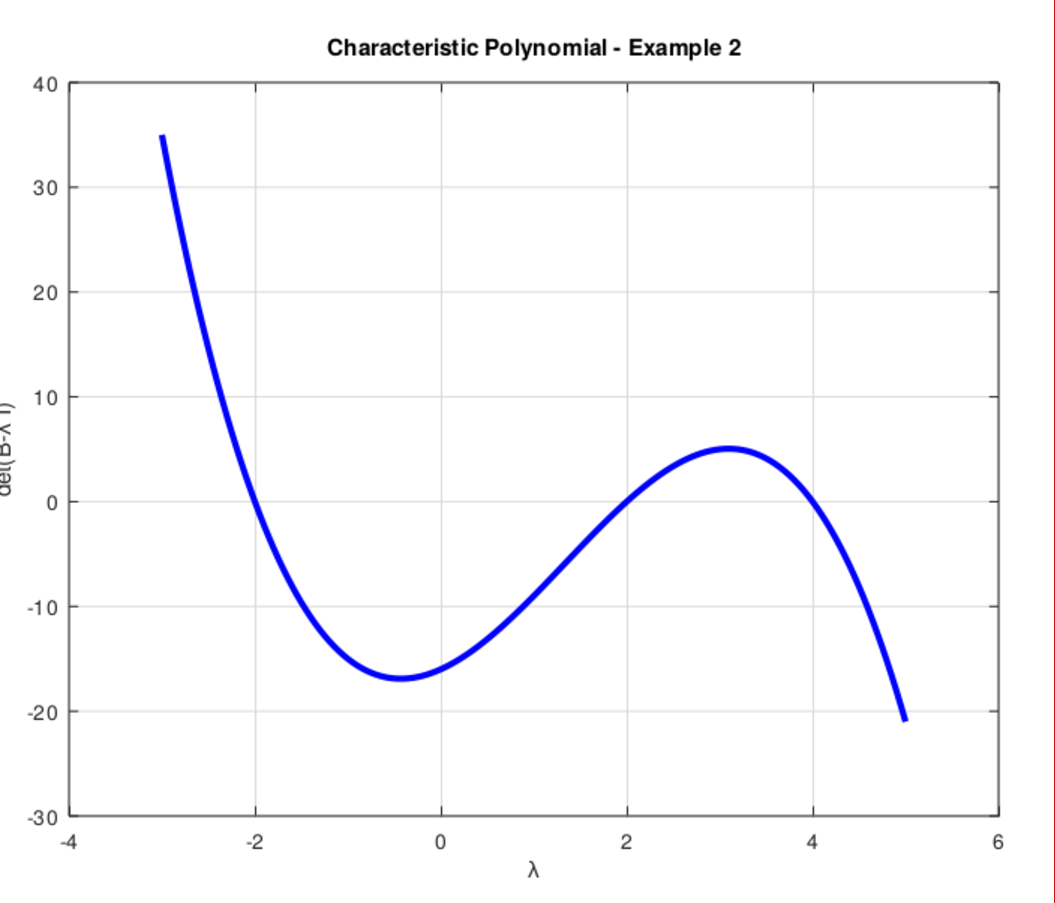
\includegraphics[width=15em]{characteristicPoly-Ex2}}
      \only<4->{\dotfield{42}{18}}
    \end{columns}

  \dotfield{60}{24}
  
\end{frame}

\section{Triangular Matrices}

\begin{frame}{Triangular Matrices}

  Recall, the determinant of a triangular matrix is the product of the
  diagonal entries.
  \begin{eqnarray*}
    C & = &
            \left[
            \begin{array}{rrrrrr}
              a_{11} & a_{12} & a_{1,3} & \cdots & a_{1,n-1} & a_{1,n} \\
              0     & a_{22} & a_{2,3} & \cdots & a_{2,n-1} & a_{2,n} \\
              0     & 0     & a_{3,3} & \cdots & a_{3,n-1} & a_{3,n} \\
                    &       &        & \ddots & \vdots   & \vdots \\
                    &       &        &        &          & a_{n,n}
            \end{array}
            \right]
  \end{eqnarray*}

  \begin{eqnarray*}
    \det(C) & = & a_{11} \cdot a_{22} \cdot a_{33} \cdots a_{n,n}.
  \end{eqnarray*}
  
\end{frame}

\begin{frame}{So What?}

  Determine the eigenvalues of the matrix
  \begin{eqnarray*}
    D & = &
            \left[
            \begin{array}{rrrrr}
              3 &  8 & -1007 & 99   & 13 \\
              0 & -4 & 1.11  & 33   & 12 \\
              0 &  0 & 21.1  & 11   & 11 \\
              0 &  0 &    0  & 3.66 & 10 \\
              0 &  0 &    0  &    0 & 9
            \end{array}
            \right]
  \end{eqnarray*}

  \uncover<2->{
      \begin{eqnarray*}
        D-\lambda I_5 & = &
            \left[
            \begin{array}{rrrrr}
              3-\lambda &  8 & -1007 & 99   & 13 \\
              0 & -4-\lambda & 1.11  & 33   & 12 \\
              0 &  0 & 21.1-\lambda  & 11   & 11 \\
              0 &  0 &    0  & 3.66-\lambda & 10 \\
              0 &  0 &    0  &    0 & 9-\lambda
            \end{array}
            \right]
  \end{eqnarray*}
  }

  \uncover<3->{
      \begin{eqnarray*}
        \det(D-\lambda I_5) & = & (3-\lambda) (-4-\lambda)
                                  (21.1-\lambda) (3.66-\lambda)
                                  (9-\lambda)
      \end{eqnarray*}
      }

      \dotfield{60}{10}
  
\end{frame}

\begin{frame}{So What?}

  Determine the eigenvalues of the matrix
  \begin{eqnarray*}
    D & = &
            \left[
            \begin{array}{rrrrr}
              3 &  8 & -1007 & 99   & 13 \\
              0 & -4 & 1.11  & 33   & 12 \\
              0 &  0 & 21.1  & 11   & 11 \\
              0 &  0 &    0  & 3.66 & 10 \\
              0 &  0 &    0  &    0 & 9
            \end{array}
            \right]
  \end{eqnarray*}

  \dotfield{60}{24}
  
\end{frame}

\section{Trace Of A Matrix}

\begin{frame}{Trace Of A Matrix}

    \begin{eqnarray*}
      E & = &
            \left[
            \begin{array}{rrrrrr}
              \textcolor{blue}{a_{11}} & a_{12} & a_{1,3} & \cdots & a_{1,n-1} & a_{1,n} \\
              a_{21} & \textcolor{blue}{a_{22}} & a_{2,3} & \cdots & a_{2,n-1} & a_{2,n} \\
              a_{31} & a_{32} & \textcolor{blue}{a_{3,3}} & \cdots & a_{3,n-1} & a_{3,n} \\
              \vdots & \vdots & \vdots & \vdots & \vdots   & \vdots \\
              a_{n1} & a_{n2} & a_{n3} &        & a_{n-1,n-1} & \textcolor{blue}{a_{n,n}}
            \end{array}
            \right]
    \end{eqnarray*}

    \begin{eqnarray*}
      \Tr(E) & = & a_{11} + a_{22} + a_{33} + \cdots + a_{n,n}.
    \end{eqnarray*}


\end{frame}

  \begin{frame}{Example}

  Determine the trace of the matrix
  \begin{eqnarray*}
    F & = &
            \left[
            \begin{array}{rrrrr}
               2 &  1 & -707  & 212  & -3 \\
              -5 & -3 & 12.2  & 409  & -4 \\
              10 &  0 &  7.1  & 409  & -5 \\
               3 &  2 &    1  & 3.00 & -6 \\
              44 &  4 &  -44  & 4444 & -7
            \end{array}
            \right]
  \end{eqnarray*}

  \dotfield{60}{24}
  
\end{frame}


\begin{frame}{So What?}

  Sometimes it just shows up!

  Example: (SPECIAL CASE!) Determine the eigenvalues of a $2\times 2$ matrix:
  \begin{eqnarray*}
    G & = & \twoByTwo{a}{b}{c}{d}.
  \end{eqnarray*}

  \only<1>{\dotfield{60}{24}}
  \only<2>{
    \begin{eqnarray*}
      \det(G-\lambda I_2) & = & \lambda^2 - \Tr(G)\lambda + \det(G).
    \end{eqnarray*}
    }
  
\end{frame}

\begin{frame}{Example}
  Determine the eigenvalues of the matrix
  \begin{eqnarray*}
    H & = & \twoByTwo{7}{8}{3}{1}.
  \end{eqnarray*}

  \dotfield{60}{24}
    
\end{frame}

\begin{frame}{Example}
  Determine the eigenvalues of the matrix
  \begin{eqnarray*}
    H & = & \twoByTwo{7}{8}{-9}{1}.
  \end{eqnarray*}

  \dotfield{60}{24}
    
\end{frame}


%\section{Examples}

\begin{frame}{Blank Page}
  \dotfield{60}{24}
\end{frame}


\end{document}
